% begin module limits-infinite-def
\begin{frame}
This definition captures the behavior of $f(x) = 1/x^2$ from Example 8:
\begin{definition}[Infinite Limit]
Let $f$ be a function defined on both sides of $a$, except perhaps at $a$ itself.  Then
\[
\lim_{x\rightarrow a}f(x) = \infty 
\]
means the values of $f(x)$ can be made arbitrarily large by taking $x$ sufficiently close to $a$, but not equal to $a$.
\end{definition}
\begin{columns}[c]
\column{.4\textwidth}
\ 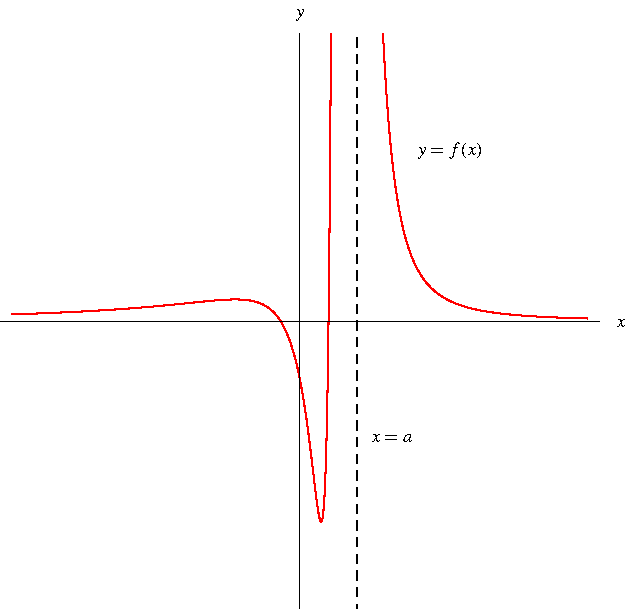
\includegraphics[height=4cm]{limits/pictures/02-02-posinf.pdf}%
\column{.6\textwidth}
\begin{itemize}
\item<2->  Other notation: $f(x) \rightarrow \infty $ as $x\rightarrow a$.
\item<3->  In such cases, the limit does not exist.
\item<4->  $\infty$ is not a number.  The notation $\lim_{x\rightarrow a}f(x) = \infty$ just expresses the particular way in which the limit doesn't exist.
\end{itemize}
\end{columns}
\end{frame}




\begin{frame}
A similar definition exists for functions that take large negative values:
\begin{definition}[Infinite Limit]
Let $f$ be a function defined on both sides of $a$, except perhaps at $a$ itself.  Then
\[
\lim_{x\rightarrow a}f(x) = -\infty 
\]
means the values of $f(x)$ can be made arbitrarily large negative by taking $x$ sufficiently close to $a$, but not equal to $a$.
\end{definition}
\begin{columns}[c]
\column{.4\textwidth}
\ 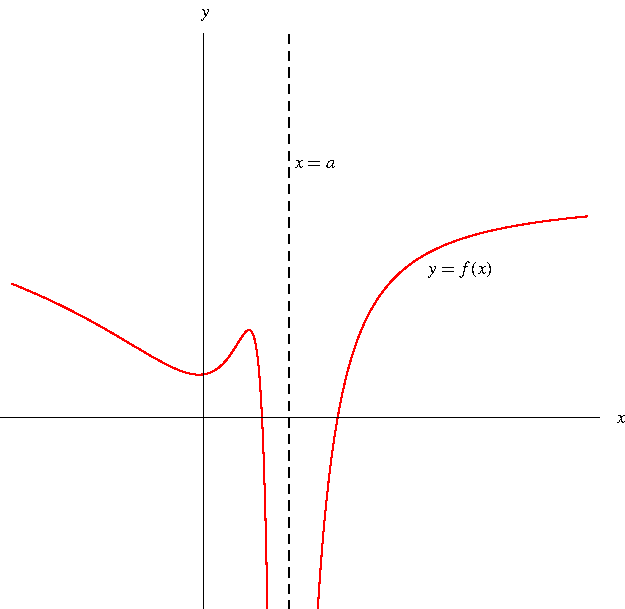
\includegraphics[height=4cm]{limits/pictures/02-02-neginf.pdf}%
\column{.6\textwidth}
\begin{itemize}
\item<2->  ``Large negative'' means the number is negative, but its absolute value is large.
\item<3->  In such cases, the limit does not exist.
\item<4->  $-\infty$ is not a number.  The notation $\lim_{x\rightarrow a}f(x) = -\infty$ just expresses the particular way in which the limit doesn't exist.
\end{itemize}
\end{columns}
\end{frame}


\begin{frame}
There are similar definitions for one-sided limits:
\begin{tabular}{ccp{3cm}}
\begin{tabular}[c]{c}{\ 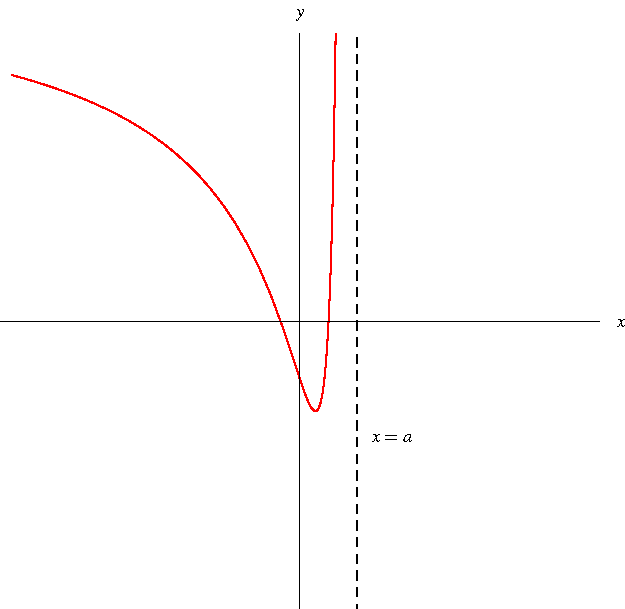
\includegraphics[height=3.2cm]{limits/pictures/02-02-posleft.pdf}}\end{tabular} &%
\begin{tabular}[c]{c}{\ 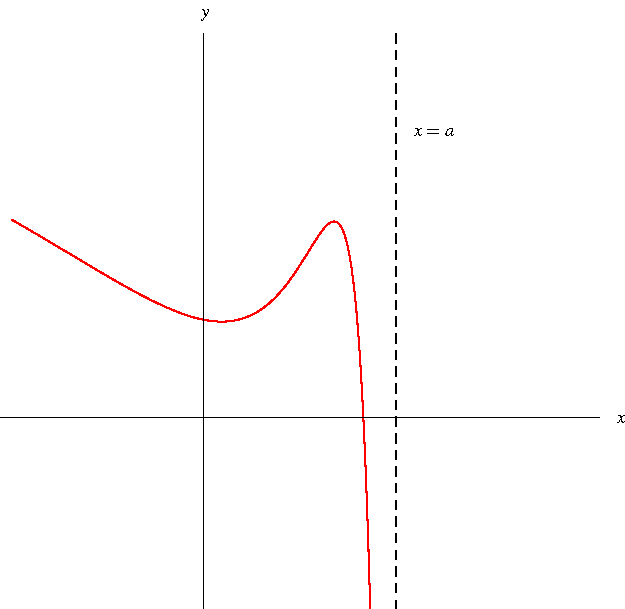
\includegraphics[height=3.2cm]{limits/pictures/02-02-negleft.pdf}}\end{tabular} &%
$x\rightarrow a^-$ means we only consider $x < a$.\\
$\lim_{x\rightarrow a^-}f(x) = \infty$  & $\lim_{x\rightarrow a^-} f(x) = -\infty$ & \\
\begin{tabular}[c]{c}{\ 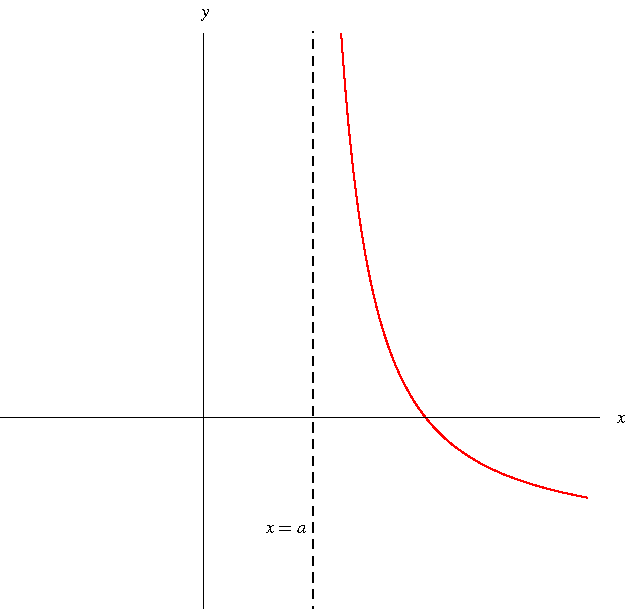
\includegraphics[height=3.2cm]{limits/pictures/02-02-posright.pdf}}\end{tabular} &%
\begin{tabular}[c]{c}{\ 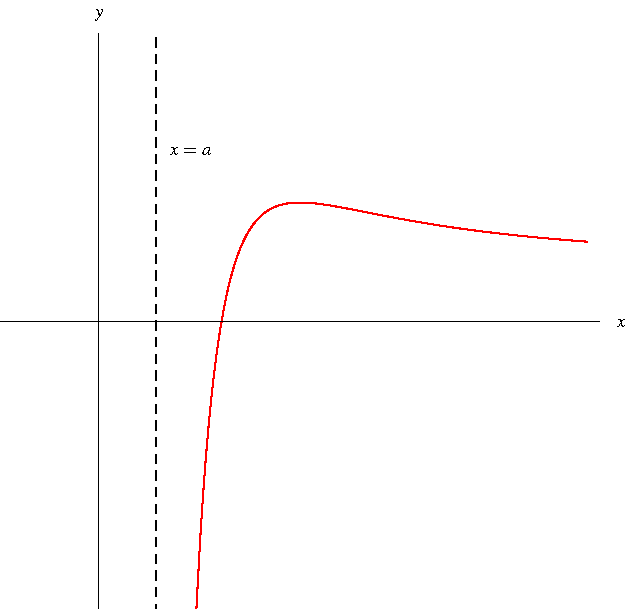
\includegraphics[height=3.2cm]{limits/pictures/02-02-negright.pdf}}\end{tabular} &%
$x\rightarrow a^+$ means we only consider $x > a$.\\
$\lim_{x\rightarrow a^+}f(x) = \infty$  & $\lim_{x\rightarrow a^+} f(x) = -\infty$ & \\
\end{tabular}
\end{frame}
% end module limits-infinite-def
